\documentclass[final,inline,narroweqnarray,a4paper]{ieee}
% In order to use the figure-defining commands in ieeefig.sty...
\usepackage{ieeefig}
\usepackage[utf8]{inputenc}
\usepackage[spanish]{babel}
\usepackage[T1]{fontenc}
\usepackage{graphicx}
\usepackage{textcomp}
\usepackage{float}
%\usepackage{hyperref}

\begin{document}

%----------------------------------------------------------------------
% Title Information, Abstract and Keywords
%----------------------------------------------------------------------
\title[TP1: Wiretapping]{%
Trabajo Práctico \textnumero 1: Wiretapping}

% format author this way for journal articles.
\author[Alvaro, Barbeito, Brum, Nievas]{%
	Alvaro Jose Fernando, 
    \authorinfo{%
    Alvaro Jose Fernando, LU: \mbox{89/10}, email: \mbox{fer1578@gmail.com}}
	\and
	Barbeito Nicolás,
    \authorinfo{%
    Barbeito Nicolás, LU: \mbox{147/10}, email: \mbox{nicolasbarbeiton@gmail.com}}
	\and
	Brum Raúl,
    \authorinfo{%
    Brum Raúl, LU: \mbox{199/98}, email: \mbox{brumraul@gmail.com}}
	\and
	Nievas Yésica
    \authorinfo{%
    Nievas Yésica, LU: \mbox{340/05}, email: \mbox{yesica.nievas@gmail.com}}
}

% make the title
\maketitle

% do the abstract
\begin{abstract}
Our premise is ...
\end{abstract}

\section{Introducción}\label{sec:intro}

\subsection{Paquetes ARP}
El protocolo ARP (Address Resolution Protocol) permite mapear direcciones de nivel de red a direcciones físicas. La idea de este protocolo se basa en el envío de paquetes que pueden ser de preguntas o respuestas. El emisor del paquete que pregunta por una dirección, envía un mensaje broadcast sobre la red local, siendo respondido por un mensaje unicast por aquel al que pertenece la dirección consultada. Mediante el envío de estos paquetes ARP se construyen las tablas que mapean direcciones de red con direcciones físicas.

\subsection{Entropía de una fuente}
Para poder definir la entropía de una fuente, necesitamos la definición de información que aportan los símbolos emitidos por dicha fuente. Se define información de un símbolo \textit{s} como 
\begin{center}
	I (\textit{s}) = log(1/P(\textit{s})) 
\end{center}
siendo P(\textit{s}) la probabilidad de ocurrencia de dicho símbolo.
De esta manera, puede calcularse la información media suministrada por una fuente de información de memoria nula (los símbolos emitidos son estadísticamente independientes) como 

\begin{center}
$\sum_{S} P(s_{i})I(s_{i}) \forall{s_{i}} \in{S}$
\end{center}

\begin{flushleft}
	Esta cantidad media de información por símbolo de la fuente, recibe el nombre de \textit{entropía} H(S) de la fuente de memoria nula.
\end{flushleft}

\begin{center}
	$H(S) =\sum_{S} P(s_{i})log(1/P(s_{i}))$ 

\end{center}
	
Debido a que la entropía de una fuente depende de la probabilidad de los diferentes símbolos que la componen, se puede demostrar que para una fuente de información de memoria nula con un alfabeto de q símbolos, el valor máximo de la entropía es precisamente log q, alcanzándose solamente si todos los símbolos son equiprobables.


\subsection{Fuente S} \label{ssec:fuenteS}

Sea P la fuente de información generada a partir de todos los paquetes Ethernet que se transmiten en una determinada red entre los instantes de tiempo $[t_{i}, t_{f}]$:

	$P_{ti,tf} = \{p_{1}...p_{n}\}$ 

\begin{flushleft}
	siendo p{\scriptsize \textit{i}} el i-ésimo paquete transmitido en la red entre los instantes de tiempo $[t_{i},t_{f}]$.
\end{flushleft}

Los paquetes $p{\scriptsize \textit{i}}$ pertenecientes a P encapsulan diferentes protocolos, que se pueden identificar a través del campo type del frame de capa 2 (p.type en Scapy). Por lo tanto, con el objetivo de distinguir los protocolos utilizados en una red, se define otra fuente de información S de la siguiente manera:

$S_{ti,tf} = \{s_{1}...s_{n}\}$ 

\begin{flushleft}
	siendo s{\scriptsize \textit{i}} = p{\scriptsize \textit{i}}.type /p{\scriptsize \textit{i}} perteneciente a P entre los instantes de tiempo $[t_{i},t_{f}]$.
\end{flushleft}


\subsection{Propuesta de una nueva fuente S{\scriptsize 1}} \label{ssec:fuenteS1}
Para analizar la entropía de la red en base a los paquetes ARP observados realizamos una nueva tool en base a la anterior que nos permitiera obtener datos de los campos de dichos paquetes. 
	Se propone como nueva fuente S1 el conjunto de símbolos conformado por las distintas direcciones IP destino:\\
	
	
		S{\scriptsize 1} = \{s{\scriptsize 1}{\tiny 1}...s{\scriptsize 1}{\tiny n}\} siendo s{\scriptsize 1}{\tiny i} el valor del campo \textit{pdst} correspondiente a la ip destino del paquete\\
		
	
	Al igual que para la fuente S, realizamos el cálculo de la entropía como fue requerido, como la probabilidad e información de sus símbolos.  

\section{Métodos y condiciones de cada experimento}

En esta sección describiremos brevemente las redes elegidas para realizar las escuchas mediante las herramientas indicadas en el enunciado del trabajo practico.

\subsection{Home Lan}

Esta medición fue realizada en la Lan de una casa por un intervalo de 2 horas. La misma cuenta con una computadora corriendo un sistema operativo Linux la cual es el router de la Lan y provee a las demás computadoras de acceso a internet ademas de otros servicios de red (proxy, dns, dhcpcd, etc). A la misma se encuentran conectadas mediante un switch 4 computadoras cableadas y 2 access point inalambricos. A estos últimos se encontraban conectados al momento de la medición una notebook y varios celulares. Ademas una de las computadoras cableadas corre una maquina virtual con ip propia independiente y otra de las computadoras cableadas posee otro isp para conectarse a internet por lo que no utiliza a la primera computadora como gateway.

\subsection{red 2}
\subsection{red 3}
\subsection{red 4}

\section{Resultados y Análisis}
En esta sección mostraremos y analizaremos los resultados obtenidos en las mediciones realizadas en las distintas redes tanto para la fuente $S$ y $S_1$ descriptas en la sección ~\ref{sec:intro} ~\ref{ssec:fuenteS} y ~\ref{ssec:fuenteS1}. Para cada una de las redes veremos sus protocolos distinguidos, la proporción de paquetes ARP en el trafico de la red y los nodos (representados por ip) distinguidos. Cabe aclarar que para la fuente $S_1$ podemos ver todos los pedidos ``who has'' de ARP ya que todas las maquinas están en el mismo dominio de broadcast pero solo podremos ver las respuestas ``is at'' de aquellas maquinas que se encuentren en igual dominio de colisión (generalmente las conectadas por wireless ya que las cableadas al estar conectadas por switches no tienen colisión y solo el destinatario recibirá la respuesta). 


\subsection{Home Lan}
\subsubsection{Fuente S}

Los resultados obtenidos para la fuente $S$ fueron:

\begin{table}[H]
    \begin{center}
        \begin{tabular}{|c|c|c|}
            \hline
            \textbf{Protocolo} & \textbf{Información} & \textbf{Probabilidad} \\ \hline
            \texttt{EAPOL     }& 12.31       & 0.01\%     \\ \hline
            \texttt{ARP       }& 5.11        & 2.88\%     \\ \hline
            \texttt{IPv6      }& 4.22        & 5.33\%     \\ \hline
            \texttt{IPv4      }& 0.12        & 91.76\%    \\ \hline
        \end{tabular}
        \caption{Home Lan - Protocolos}
        \label{table:homelanS}
    \end{center}
\end{table}

Como puede observarse en la figura~\ref{torta:homelanS} el protocolo mas utilizado es IPv4 en un 91.76\% mientras que IPv6 y ARP solo son utilizados en un 5.33\% y 2.88\% respectivamente. EAPOL (autenticación wireless) no tiene prácticamente incidencia.
Observamos ademas que el protocolo ARP tiene solo una incidencia del 2.88\% en el trafico total de la fuente lo que hace que el overhead aportado por el mismo no sea significativo. 

\begin{figure}[H]
    \begin{center}
        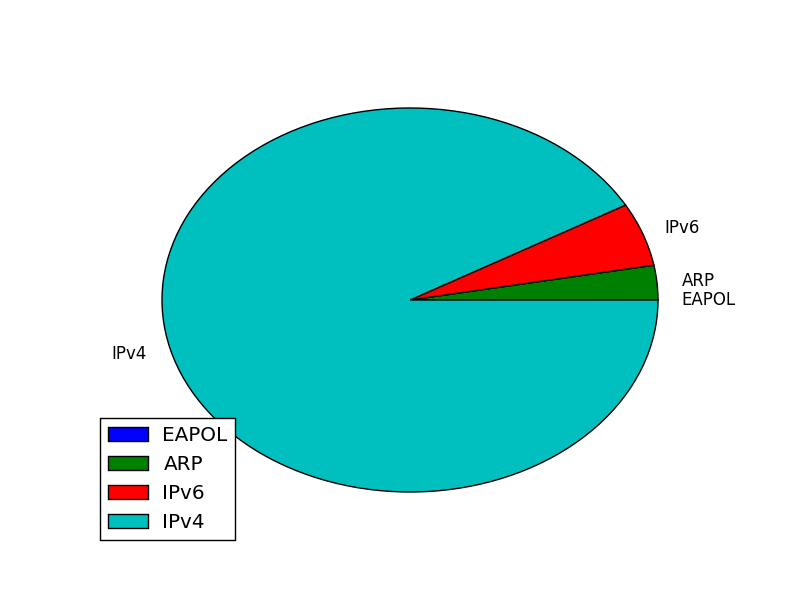
\includegraphics[width=0.5\textwidth]{plot/homelanS-pie.png}
        \caption{Home Lan - Probabilidades}
        \label{torta:homelanS}
    \end{center}
\end{figure}

Por otro lado la entropía de la fuente $S$ fue de 0.4892 lo que hace que los símbolos emitidos por la fuente $S$ sean muy previsibles. Esto podemos notarlo en la figura~\ref{histo:homelanS} donde observamos que el protocolo con mayor porcentaje de aparición, IPv4,  sea el que menos información aporta a la fuente. La información aportada por este se encuentra por debajo de la entropía de $S$. Como contraste observamos en la figura~\ref{histo:homelanS} que el protocolo EAPOL es el que mas información aporta pero según lo observado en la figura~\ref{torta:homelanS} tiene una probabilidad muy baja lo que hace que no incida en la entropía.

\begin{figure}[H]
    \begin{center}
        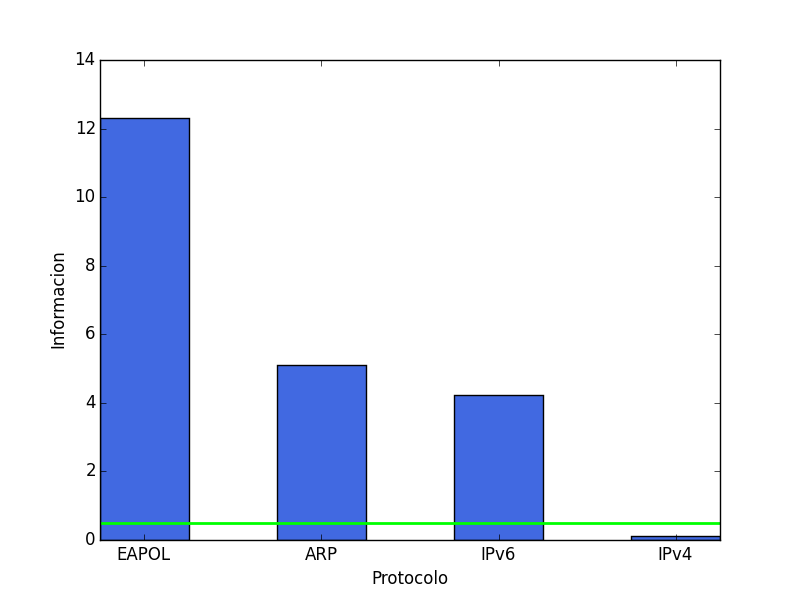
\includegraphics[width=0.5\textwidth]{plot/homelanS-bar.png}
        \caption{Home Lan - Información}
        \label{histo:homelanS}
    \end{center}
\end{figure}

\subsubsection{Fuente $S_1$}
Para la fuente $S_1$ expondremos las ip de destino, los resultados fueron :

\begin{table}[H]
    \begin{center}
        \begin{tabular}{|c|c|c|}
            \hline
            \textbf{Protocolo} & \textbf{Información} & \textbf{Probabilidad} \\ \hline
            \texttt{192.168.10.10}&7.68        & 0.48\%     \\ \hline
            \texttt{192.168.10.27}&6.41        & 1.16\%     \\ \hline
            \texttt{192.168.10.11}&6.30        & 1.26\%     \\ \hline
            \texttt{192.168.10.13}&5.09        & 2.92\%     \\ \hline
            \texttt{192.168.10.7}&4.33         & 4.97\%     \\ \hline
            \texttt{192.168.10.1}&4.00         & 6.23\%     \\ \hline
            \texttt{192.168.10.4}&2.54         & 17.15\%    \\ \hline
            \texttt{192.168.10.6}&2.11         & 23.09\%    \\ \hline
            \texttt{192.168.10.9}&1.22         & 42.69\%    \\ \hline
        \end{tabular}
        \caption{Home Lan - Nodos}
        \label{table:homelanS1}
    \end{center}
\end{table}

Como puede observarse en la figura~\ref{torta:homelanS1} las ip que aparecen con mayor frecuencia como destino en los paquetes ARP son la ``192.168.10.9'' en un 42.69\%, la ``192.168.10.6'' en un 23.09\% y la ``192.168.10.4'' en un 17.15\% por lo que estas serán los nodos distinguidos de la fuente y las que menos información aporten.

\begin{figure}[H]
    \begin{center}
        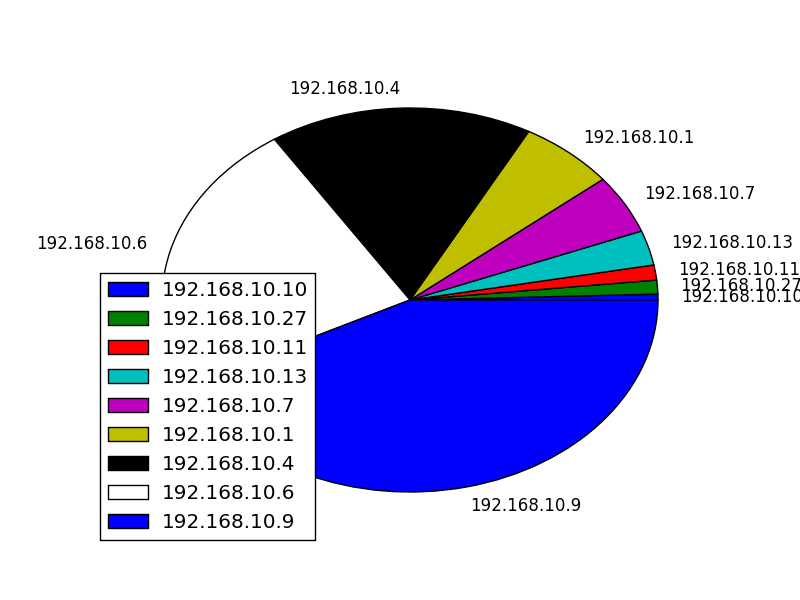
\includegraphics[width=0.5\textwidth]{plot/homelanS1-pie.png}
        \caption{Home Lan - Probabilidades}
        \label{torta:homelanS1}
    \end{center}
\end{figure} 

La entropía de la fuente $S_1$ fue de 2.25. En la figura~\ref{histo:homelanS1} se observa la información aportada por los distintos nodos y como 2 de los nodos distinguidos quedan por debajo de la entropía de la fuente y el otro apenas por arriba. 

\begin{figure}[H]
    \begin{center}
        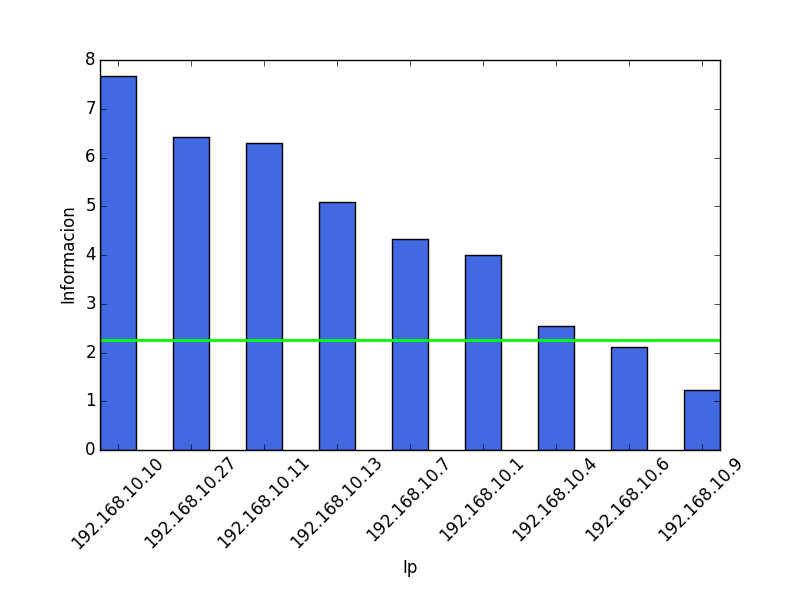
\includegraphics[width=0.5\textwidth]{plot/homelanS1-bar.png}
        \caption{Home Lan - Información}
        \label{histo:homelanS1}
    \end{center}
\end{figure}

En el análisis de la fuente $S_1$ vemos que ninguno de los 3 nodos distinguidos pertenecen al router de la red, la ip ``192.168.10.1''. De los nodos distinguidos las ip ``192.168.10.6'' y ``192.168.10.4'' se explican ya que la primera es la notebook que realizo la captura en la red y la segunda es la computadora que la controlaba remotamente mediante SSH. La ip ``192.168.10.9'' corresponde a la ip de una consola de video juegos la cual se encontraba apagada al momento de realizar la captura, en la ip ``192.168.10.4'' hay un daemon ejecutándose que se comunica con la consola de video juegos. Al estar esta apagada hay muchos pedidos ``who has 192.168.10.9'' y ninguna respuesta por lo que los pedidos son reiterados varias veces incrementado su incidencia. 

\section{Conclusión}

\section{Referencias}

\end{document}
